\documentclass[sigconf,screen,nonacm]{acmart}

% --- ACM metadata cleanup for course-project use ---
\settopmatter{printacmref=false}
\renewcommand\footnotetextcopyrightpermission[1]{}
\pagestyle{plain}
\setcopyright{none}

% --- Project metadata ---
\newcommand{\ProjectTitle}{From Linear Scores to a Single Hidden Layer: A Mathematical Study of Simple Learning Systems}
\newcommand{\CourseName}{National AI Center --- AI Academy}
\newcommand{\ProjectType}{Math4AI Final Capstone Project}

% --- Packages ---
\usepackage{amsmath, amssymb, booktabs, enumitem, hyperref, graphicx}

% --- Inline macro definitions (replaces missing macros.tex) ---
\newcommand{\vx}{\mathbf{x}}
\newcommand{\vs}{\mathbf{s}}
\newcommand{\vh}{\mathbf{h}}
\newcommand{\vb}{\mathbf{b}}
\newcommand{\vone}{\mathbf{1}}
\newcommand{\vbone}{\mathbf{b}^{(1)}}
\newcommand{\vbtwo}{\mathbf{b}^{(2)}}
\newcommand{\mW}{\mathbf{W}}
\newcommand{\mWone}{\mathbf{W}^{(1)}}
\newcommand{\mWtwo}{\mathbf{W}^{(2)}}
\newcommand{\mX}{\mathbf{X}}
\newcommand{\mH}{\mathbf{H}}
\newcommand{\mS}{\mathbf{S}}
\newcommand{\mP}{\mathbf{P}}
\newcommand{\mY}{\mathbf{Y}}
\newcommand{\mZ}{\mathbf{Z}}
\newcommand{\R}{\mathbb{R}}
\newcommand{\loss}{\mathcal{L}}
\newcommand{\tanhact}{\tanh}
\newcommand{\softmaxrow}{\mathrm{softmax}}

% --- PDF metadata ---
\hypersetup{
  pdftitle={\ProjectTitle},
  pdfauthor={Student Team},
  pdfsubject={Math4AI Capstone Report},
  pdfkeywords={softmax regression, neural networks, backpropagation, cross-entropy, classification, NumPy}
}

\title{\ProjectTitle}
\subtitle{\ProjectType}

\author{Ziyad Muradov}
\affiliation{%
  \institution{\CourseName}
  \country{Azerbaijan}
}
\email{ziyad.muradov25@aiacademy.az}

\author{Emin Huseynli}
\affiliation{%
  \institution{\CourseName}
  \country{Azerbaijan}
}
\email{emin.huseynli25@aiacademy.az}

\author{Ismayil Yusifli}
\affiliation{%
  \institution{\CourseName}
  \country{Azerbaijan}
}
\email{ismayil.yusifli25@aiacademy.az}

\author{Kamal Soltanaliyev}
\affiliation{%
  \institution{\CourseName}
  \country{Azerbaijan}
}
\email{kamal.soltaneliyev25@aiacademy.az}

\begin{document}

\begin{abstract}
This report studies when a one-hidden-layer nonlinear classifier meaningfully improves on a linear decision rule, and when additional model complexity is unnecessary. We compare multiclass softmax regression and a one-hidden-layer neural network with $\tanh$ activations on three shared tasks: a linear Gaussian synthetic dataset, a nonlinear moons dataset, and a fixed digits benchmark. Our analysis combines mathematical derivations, controlled experiments, required ablations, failure-case analysis, prediction of reliability and confidence, and repeated-seed evaluation to determine where linear geometry is sufficient, where nonlinear representation changes the problem, and what limitations remain.
\end{abstract}

\keywords{softmax regression, neural networks, backpropagation, cross-entropy, classification, NumPy}

\maketitle

% ============================================================
\section{Introduction / Framing}
% ============================================================

The main purpose of this capstone project is to implement multiclass softmax regression and a one-hidden-layer nonlinear classifier on three different datasets, in order to determine when a one-hidden-layer neural network genuinely improves upon a linear decision rule and when additional model complexity is unnecessary.
Contrary to common belief, neural networks do not always outperform baseline models in all cases. Therefore, the goal is to identify---through both mathematical analysis and empirical evidence---when increased representational capacity is truly justified.

Softmax regression is a linear classifier that computes class scores using a linear function of the input and the decision boundaries it produces are straight lines in 2D or hyperplanes in higher dimensions. Therefore, softmax regression performs well on datasets where class separation is approximately linear, but it fails on datasets with inherently nonlinear structure.

A single-hidden-layer neural network extends the linear model by incorporating a nonlinear transformation via a hidden layer. This architecture maps the input data into a higher-dimensional feature space, enabling the model to resolve patterns that are not linearly separable in their original state. While this increased representational capacity allows the model to approximate sophisticated functions, the added flexibility simultaneously introduces significant computational and optimization complexity.

In order to justify additional complexity of neural network compared to softmax regression, they should be performed on given datasets in this capstone with same training, validation and test splits as well as same optimization approaches and evaluation metrics.

\paragraph{Contributions.}
A clean introduction usually ends with 3--5 concrete contributions. For this project, strong contributions often include:
\begin{enumerate}[leftmargin=*,itemsep=0.25em]
    \item Derivation of softmax cross-entropy as negative log-likelihood.
    \item Conceptual explanation of backpropagation followed by a full gradient derivation for the one-hidden-layer network.
    \item Controlled comparison of a linear model and a nonlinear model on datasets with distinct geometric structure.
    \item Interpretation of required ablations, one failure case, and repeated-seed statistics on the digits benchmark.
\end{enumerate}

\paragraph{Preview of findings.}
In our experiments, the linear model is expected to be highly competitive on the Gaussian task because the class geometry is well matched to an affine separator. On the moon's task, the hidden layer is expected to provide a meaningful representational change because a nonlinear boundary is needed. On the digits benchmark, the comparison should be interpreted using both accuracy and cross-entropy, with model selection based on validation cross-entropy and final uncertainty quantified via repeated-seed statistics.

% ============================================================
\section{Background and Mathematical Setup}
% ============================================================

\subsection{Supervised classification and data splits}
A supervised learning dataset is defined as a collection of $N$ independent and identically distributed (i.i.d.) observations:
\[
\mathcal{D} = \{(\mathbf{x}^{(i)}, y^{(i)})\}_{i=1}^{N}
\]

\noindent
$\mathbf{x}^{(i)} \in \mathbb{R}^{d}$ represents the $i$-th input feature vector in a $d$-dimensional space.

\noindent
$y^{(i)}$ represents the ground-truth label (e.g., $y \in \{0, 1, \dots, C-1\}$ for a $C$-class classification task).

\noindent
The objective is to learn a function $f(\mathbf{x}; \theta)$, parameterized by $\theta$, that accurately predicts the label $y$ for unseen inputs by minimizing a loss function
\[
\mathcal{L}\!\big(f(\mathbf{x}; \theta),\, y\big).
\]

The dataset $\mathcal{D}$ is partitioned into three mutually exclusive subsets: training, validation, and test data.

\medskip\noindent\textbf{Training set.} Used to learn the model parameters through forward propagation and backpropagation (gradient descent). The parameters are iteratively updated to minimize the loss function.

\medskip\noindent\textbf{Validation set.} Used as unseen data to guide model selection and tune hyperparameters. It provides an unbiased estimate of model performance during development and helps prevent overfitting.

\medskip\noindent\textbf{Test set.} Strictly reserved for final evaluation to measure the generalization performance of the model. The test set must not be used in any way to influence model training or hyperparameter selection.

\subsection{Softmax regression}
For input $\vx \in \R^d$ and $k$ classes, the linear model computes logits
\begin{equation}
    \vs(\vx) = \mW \vx + \vb,
\end{equation}
where $\mW \in \R^{k \times d}$ and $\vb \in \R^k$. The softmax map converts logits to probabilities:
\begin{equation}
    p_j(\vx) = \frac{\exp(s_j(\vx))}{\sum_{\ell=1}^{k} \exp(s_{\ell}(\vx))}.
\end{equation}

The predicted class is the argmax of $\vs(\vx)$. The decision boundary between two classes $i$ and $j$ satisfies:
\begin{equation}
\left(\mathbf{w}_i - \mathbf{w}_j\right)^{\top} \mathbf{x} + \left(b_i - b_j\right) = 0,
\end{equation}
which is an affine equation, so decision boundaries are straight lines in 2D, planes in 3D, and hyperplanes in general. Consequently, softmax regression performs well on linearly separable data but cannot represent curved boundaries.

\subsection{Cross-entropy as negative log-likelihood}

For each training example $(\mathbf{x}^{(i)}, y^{(i)})$, the predicted probability is $p(y^{(i)} \mid \mathbf{x}^{(i)}; \theta)$.
The likelihood function over the dataset is:
\begin{equation}
L(\theta) = \prod_{i=1}^{n} p\!\left(y^{(i)} \mid \mathbf{x}^{(i)}; \theta\right).
\end{equation}

Taking the logarithm to avoid numerical underflow:
\begin{equation}
\ell(\theta) = \sum_{i=1}^{n} \log p\!\left(y^{(i)} \mid \mathbf{x}^{(i)}; \theta\right).
\end{equation}

We minimize the negative average log-likelihood:
\begin{equation}
J(\theta) = -\frac{1}{n}\,\ell(\theta)
= -\frac{1}{n} \sum_{i=1}^{n} \log p\!\left(y^{(i)} \mid \mathbf{x}^{(i)}; \theta\right).
\end{equation}

This is exactly the cross-entropy loss:
\begin{equation}
J(\theta) = \frac{1}{n} \sum_{i=1}^{n} \mathcal{L}(\mathbf{x}^{(i)}, y^{(i)}),
\quad\text{where}\quad
\mathcal{L}(\mathbf{x}, y) = -\log p(y \mid \mathbf{x}; \theta).
\end{equation}

Minimizing the average cross-entropy is equivalent to maximizing the log-likelihood, adjusting $\theta$ so that the observed labels become as probable as possible under the model.

\subsection{One-hidden-layer neural network}
The nonlinear model computes:
\begin{equation}
    \vh = \tanh\!\left(\mWone \vx + \vbone\right), \qquad \vs = \mWtwo \vh + \vbtwo.
\end{equation}
The $\tanh$ activation is an S-shaped nonlinear function ranging between $-1$ and $1$; it is zero-centered, which aids convergence. While a linear model is restricted to affine decision boundaries, the hidden layer maps the input $\vx$ into a latent space $\vh$ through a nonlinear transformation, allowing the model to warp the data's original geometry so that the final softmax layer can separate classes that are inherently non-linearly separable.

\subsection{Backpropagation}
Backpropagation is the efficient, recursive application of the multivariate chain rule through a composed computational graph. During the forward pass, the model sequentially computes intermediate quantities---linear pre-activations, nonlinear hidden activations, logits, and final class probabilities---culminating in the scalar loss $\loss$. In the backward pass, the error signal is propagated in reverse order to obtain gradients for all parameters ($\mWone, \vbone, \mWtwo, \vbtwo$), reusing gradients of later layers to compute those of earlier ones.

\subsection{Gradient derivation}
For a mini-batch matrix $\mX \in \R^{n \times d}$, the vectorized forward pass is:
\begin{align}
    \mZ_{1} &= \mX\,\mWone^{\top} + \vone\,\vbone^{\top}, \\
    \mH     &= \tanh(\mZ_{1}), \\
    \mS     &= \mH\,\mWtwo^{\top} + \vone\,\vbtwo^{\top}, \\
    \mP     &= \mathrm{softmax}(\mS).
\end{align}

\paragraph{Step 1: Output layer sensitivity.}
The error signal at the output layer is:
\begin{equation}
\boldsymbol{\delta}_{2} = \frac{\partial \loss}{\partial \mS} = \frac{1}{n}(\mP - \mY).
\end{equation}
\textit{Code:} \texttt{dS = (P - Y\_onehot) / n}

\paragraph{Step 2: Gradients for output parameters.}
Using $\boldsymbol{\delta}_{2}$ and the hidden activations $\mH$:
\begin{equation}
\frac{\partial \loss}{\partial \mWtwo} = \boldsymbol{\delta}_{2}^{\top}\,\mH,
\qquad
\frac{\partial \loss}{\partial \vbtwo} = \boldsymbol{\delta}_{2}^{\top}\,\vone.
\end{equation}
\textit{Code:} \texttt{dW2 = dS.T @ H},\quad \texttt{db2 = dS.sum(axis=0)}

\paragraph{Step 3: Backpropagation through the hidden layer.}
The error signal for the first layer is obtained by propagating backward through $\mWtwo$:
\begin{equation}
\frac{\partial \loss}{\partial \mH} = {\delta}_{2}\,\mWtwo.
\end{equation}
Applying the $\tanh$ derivative $(1 - \mH^{2})$:
\begin{equation}
\boldsymbol{\delta}_{1} = \frac{\partial \loss}{\partial \mZ_{1}}
= \frac{\partial \loss}{\partial \mH} \odot (1 - \mH^{2}).
\end{equation}
\textit{Code:} \texttt{dH = dS @ W2},\quad \texttt{dZ1 = dH * (1 - H**2)}

\paragraph{Step 4: Gradients for input parameters.}
Using the input data $\mX$:
\begin{equation}
\frac{\partial \loss}{\partial \mWone} = \boldsymbol{\delta}_{1}^{\top}\,\mX,
\qquad
\frac{\partial \loss}{\partial \vbone} = \boldsymbol{\delta}_{1}^{\top}\,\vone.
\end{equation}
\textit{Code:} \texttt{dW1 = dZ1.T @ X},\quad \texttt{db1 = dZ1.sum(axis=0)}

\paragraph{Step 5: $L^{2}$ regularization.}
The gradient of the $L^{2}$ penalty $\lambda\,\mW$ is added to each weight gradient:
\begin{equation}
    \nabla_{\mW}^{\mathrm{total}} = \nabla_{\mW}^{\mathrm{data}} + \lambda\,\mW.
\end{equation}
\textit{Code:} \texttt{dW += lam * W}

\subsection{Geometric expectations for the datasets}
\label{sec:geometric}
In the Gaussian dataset, the two classes are generated from Gaussian distributions with similar covariance structures, so the log-odds between classes is an affine function of the input. The optimal decision boundary is therefore a hyperplane, and softmax regression is perfectly matched to this task; the additional nonlinear capacity of a neural network is redundant.

For the moons dataset, the two classes form interleaving crescent shapes that are not linearly separable. Any affine decision rule will cut through the crescents with high error. The one-hidden-layer neural network addresses this by using $\tanh$ to warp the input space into a representation where a linear separator suffices.

% ============================================================
\section{Methods}
% ============================================================

\subsection{Datasets}
Three datasets are used across all experiments.
\begin{itemize}[leftmargin=*]
    \item \textbf{Linear Gaussian task:} Two classes drawn from Gaussian distributions with mild overlap, forming approximately linearly separable clusters. As established in Section~\ref{sec:geometric}, softmax regression is geometrically sufficient here.
    \begin{itemize}
        \item \textbf{File:} \texttt{starter\_pack/data/linear\_gaussian.npz}
    \end{itemize}
    \item \textbf{Moons task:} A nonlinear binary classification problem where the two classes form interleaving crescent shapes that cannot be separated by a straight line. A curved boundary is required, motivating the neural network.
    \begin{itemize}
        \item \textbf{File:} \texttt{starter\_pack/data/moons.npz}
    \end{itemize}
    \item \textbf{Digits benchmark:} Multiclass classification of handwritten digit images (0--9), represented as 64-dimensional vectors ($8 \times 8$ image, flattened). Features are scaled to $[0, 1]$. A fixed train/validation/test split is provided and must be strictly followed; both accuracy and cross-entropy are reported.
    \begin{itemize}
        \item \textbf{Files:} \texttt{starter\_pack/data/digits\_data.npz}, \texttt{digits\_split\_indices.npz}
    \end{itemize}
\end{itemize}

\subsection{Models}
Two models are implemented and compared:
\begin{itemize}[leftmargin=*]
    \item Multiclass softmax regression.
    \item One-hidden-layer neural network with $\tanh$ hidden activations and softmax output.
\end{itemize}
The neural network uses a default hidden layer width of $h = 32$ across all primary experiments.
To investigate how model capacity affects learning on non-linear data, we conducted a systematic ablation study on the moons dataset using hidden layer widths $h \in \{2, 8, 32\}$.

\subsection{Training Protocol}

\begin{description}
    \item[Optimizer \& Learning Rate:] We employ \textbf{vanilla stochastic gradient descent (SGD)} with a fixed learning rate of $lr = 0.05$ throughout all experiments. This learning rate is applied uniformly across softmax regression, neural networks, and all datasets to ensure fair comparison.

    \item[Mini-Batching:] Training uses \textbf{mini-batch gradient descent} with batch size $B = 64$. Within each epoch, the training set is divided into non-overlapping mini-batches and shuffled (seeded for reproducibility). Gradients are averaged over the batch before weight updates.

    \item[Regularization:] \textbf{$L_2$ regularization} with coefficient $\lambda = 10^{-4}$ is applied to all learnable parameters during training. The regularization term is:
    \[
    \text{Reg} = \frac{\lambda}{2} (\|W_1\|_F^2 + \|W_2\|_F^2)
    \]
    for neural networks, and $\frac{\lambda}{2} \|W\|_F^2$ for softmax. The gradient of the $L_2$ penalty is explicitly added to computed mini-batch gradients before each weight update.

    \item[Epoch Budget:] \hfill
    \begin{itemize}
        \item \textbf{Synthetic datasets (Linear Gaussian, Moons):} 100 epochs per run.
        \item \textbf{Digits dataset:} 200 epochs per run (doubled due to higher complexity and dataset size).
    \end{itemize}

    \item[Weight Initialization:] \hfill
    \begin{itemize}
        \item \textbf{Softmax regression:} Weights initialized as $W \sim 0.01 \cdot \mathcal{N}(0, I)$, biases $b = 0$.
        \item \textbf{Neural network (1-hidden-layer):} Xavier initialization with standard deviation $\sigma_1 = \sqrt{1/(d+h)}$ for the first layer and $\sigma_2 = \sqrt{1/(h+k)}$ for the second layer, ensuring stable gradient flow.
    \end{itemize}

    \item[Numerical Stability Measures:] \hfill
    \begin{itemize}
        \item \textbf{Softmax computation:} Before exponential, logits are shifted by their max value per sample to prevent numerical overflow:
        \[
        P = \frac{\exp(S - \max(S))}{\sum \exp(S - \max(S))}
        \]
        \item \textbf{Cross-entropy loss:} Probabilities are clipped to $[10^{-12}, 1.0]$ before taking logarithms to avoid $\log(0)$.
        \item \textbf{Gradient scaling:} All gradients are scaled by $1/n$ (batch size) before weight updates, preventing scale-dependent learning rate sensitivity.
    \end{itemize}

    \item[Checkpoint Policy:] \hfill
    \begin{itemize}
        \item \textbf{Synthetic datasets:} Final weights from epoch 99 (no checkpointing).
        \item \textbf{Digits dataset:} Early stopping with \texttt{checkpoint\_on\_val = True}. The model achieving the \textbf{lowest validation cross-entropy loss} during training is selected as the final model.
    \end{itemize}

    \item[Validation Selection Metric:] Validation cross-entropy loss is the primary selection metric. It directly measures model performance on unseen data without variance contributions from accuracy (which is discrete). By minimizing validation cross-entropy, the model captures both calibration and correctness simultaneously, providing the most stable selection criterion across datasets and architectures.
\end{description}

\subsection{Evaluation Metrics}

\begin{description}
    \item[Classification Accuracy:] Accuracy is the fraction of correct predictions, defined as:
    \[
    \text{Accuracy} = \frac{1}{n} \sum_{i=1}^n \mathbb{1}(\text{argmax}_j P_{ij} = \text{argmax}_j Y_{ij})
    \]
    where $P$ is the predicted probability matrix and $Y$ is the one-hot encoded label matrix. It measures the direct correctness of the model's top prediction.

    \item[Mean Cross-Entropy Loss:] Mean cross-entropy measures the negative log-likelihood of the true labels under the predicted distribution:
    \[
    \text{Loss} = -\frac{1}{n} \sum_{i=1}^n \sum_{j=1}^k Y_{ij} \log(P_{ij})
    \]
    To ensure numerical stability, $P$ is clipped to $[10^{-12}, 1.0]$ before the logarithmic operation. The total loss evaluated during training includes this data loss plus the $L_2$ regularization term $\frac{\lambda}{2} \|W\|_F^2$.

    \item[Utility of Dual Metrics:] Reporting both metrics is essential because they provide complementary views of model performance:
    \begin{itemize}
        \item \textbf{Accuracy} is a discrete metric that identifies if the prediction is correct, but it fails to distinguish between high-confidence and low-confidence predictions.
        \item \textbf{Cross-entropy} is a continuous metric that reflects model confidence and calibration. It penalizes ``correct'' predictions that have low confidence and rewards those with high probability, offering a more nuanced view of generalization and prediction quality.
    \end{itemize}
\end{description}

\subsection{Sanity Checks}
To ensure the mathematical and structural integrity of the implementation, five sanity checks were performed, all of which passed successfully:

\begin{itemize}
    \item \textbf{Check 1: Probabilities sum to one.} Softmax outputs were verified to sum to exactly $1.0$ across all samples.
    \item \textbf{Check 2: Numerical stability.} The implementation produced no \texttt{NaN} or \texttt{Inf} values when evaluated on extreme inputs ($\pm 1000$).
    \item \textbf{Check 3: Gradient check.} Finite-difference validation confirmed the correctness of the analytical gradients, yielding a relative error of $2.02 \times 10^{-11}$.
    \item \textbf{Check 4: Loss decreases.} The optimization logic was verified by performing 20 SGD steps, during which the loss decreased from $1.0804$ to $0.9295$.
    \item \textbf{Check 5: Overfit tiny subset.} The model successfully overfit a tiny subset of 10 examples, reaching a classification accuracy of $1.0000$ within 200 epochs.
\end{itemize}
% ============================================================
\section{Experiments}
% ============================================================

\subsection{Core comparison on the linear Gaussian task}

Both models achieve identical test accuracy (95.0\%) and similar test cross-entropy loss. Softmax regression: test loss 0.1555, accuracy 95.0\%. Neural network: test loss 0.1539, accuracy 95.0\%.

\begin{figure}[htbp]
    \centering
    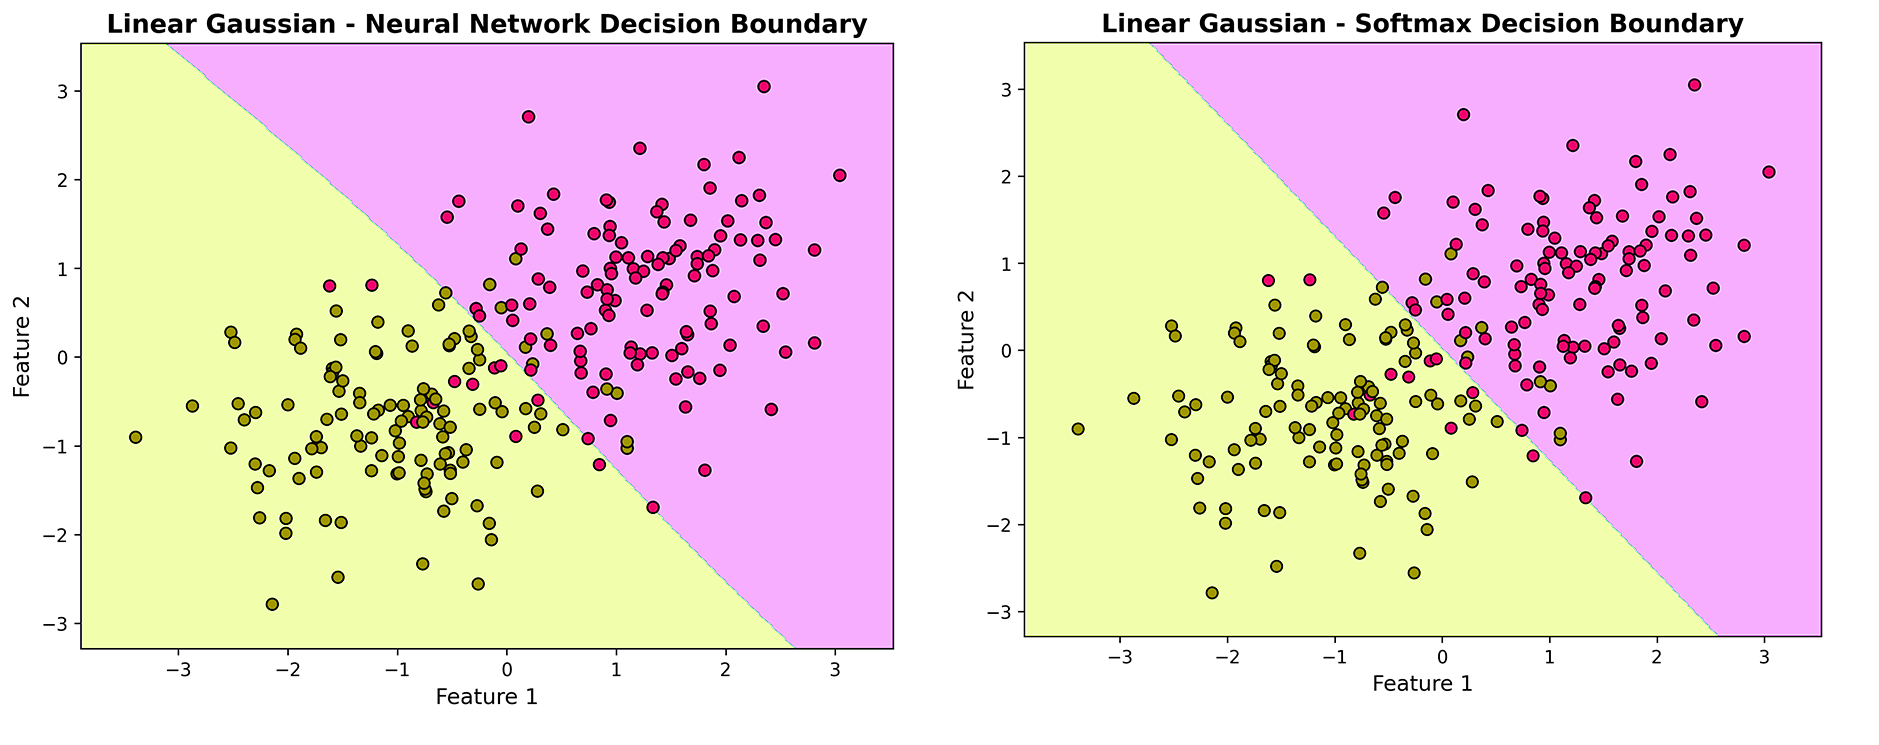
\includegraphics[width=1\linewidth]{figures/linear_gaussian.png}
    \caption{Linear Gaussian: Softmax Regression decision boundary vs One-Hidden-Layer NN decision boundary.}
    \label{fig:gaussian-softmax}
\end{figure}

\noindent\textbf{Interpretation:} Both models learn identical linear separators (Figures~\ref{fig:gaussian-softmax}, indicating the hidden layer provides no benefit on this linearly separable task. The Gaussian task is geometrically sufficient for linear models; the nonlinear hidden layer in the neural network does not improve classification. Both achieve the inherent task difficulty ceiling.

\subsection{Core comparison on the moons task}

The neural network outperforms softmax regression. Test accuracies: Softmax 83.75\%, NN 85.0\%; test losses: Softmax 0.3112, NN 0.2755.

\begin{figure}[htbp]
    \centering
    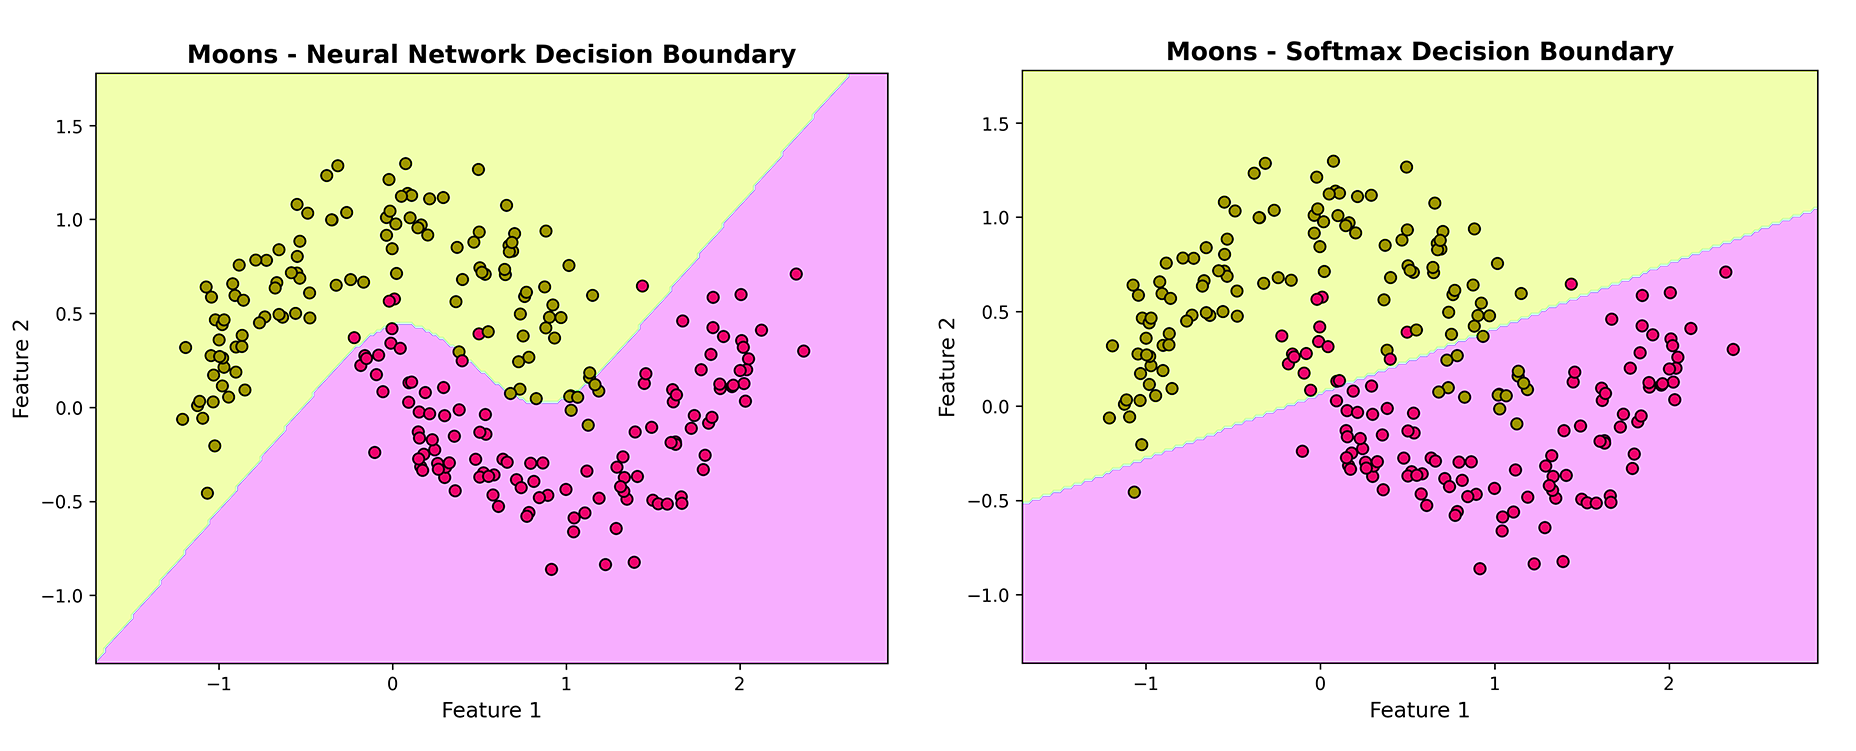
\includegraphics[width=1\linewidth]{figures/moontask.png}
    \caption{Moons: Softmax Regression decision boundary vs One-Hidden-Layer NN decision boundary}
    \label{fig:moons-softmax}
\end{figure}


\noindent\textbf{Interpretation:} The hidden layer enables the NN to learn the necessary nonlinear decision boundary (Figures~\ref{fig:moons-softmax}). The neural network effectively transforms the problem into a linearly separable one in hidden space via the tanh activation, achieving superior test performance and lower cross-entropy loss.

\subsection{Core comparison on the digits benchmark}

Model selection on digits used the early-stopping criterion: the checkpoint achieving the lowest validation cross-entropy loss. The neural network outperforms softmax regression.

\begin{table}[htbp]
    \centering
    \caption{Final digits test results from best validation checkpoint, averaged over 5 seeds.}
    \label{tab:final-results}
    \begin{tabular}{lcc}
        \toprule
        Model & Test Accuracy & Test Cross-Entropy \\
        \midrule
        Softmax Regression & $93.80\% \pm 0.23\%$ & $0.2773 \pm 0.0003$ \\
        One-Hidden-Layer NN & $94.95\% \pm 0.31\%$ & $0.1802 \pm 0.0055$ \\
        \bottomrule
    \end{tabular}
\end{table}

\noindent\textbf{Model Selection Details:} For softmax regression, the model achieved best validation loss of 0.2191 at epoch 149 (validation accuracy 94.93\%). For the neural network, best validation loss was 0.1255 at epoch 190 (validation accuracy 96.90\%). Both checkpoints were confirmed to generalize stably on the held-out test set. The NN's lower test cross-entropy (0.1816 vs.\ 0.2776) indicates better-calibrated probability estimates on unseen data.

\subsection{Required capacity ablation on moons}

We study the effect of hidden layer width $h \in \{2, 8, 32\}$ on the moons task. Figure~\ref{fig:moons-ablation} shows decision boundaries and training dynamics across all three capacities.

\begin{figure}[htbp]
    \centering
    
\includegraphics[width=0.85\linewidth]{figures/moons_ablation_comparison.png}
    \caption{Capacity ablation on Moons: decision boundaries and training curves for hidden widths $h \in \{2, 8, 32\}$.}
    \label{fig:moons-ablation}
\end{figure}

\noindent\textbf{Findings:}
\begin{itemize}
    \item \textbf{$h=2$:} Underfits. Rough, coarse decision boundary. Test accuracy $\approx 85\%$. Insufficient capacity to learn the nonlinear separation.
    \item \textbf{$h=8$:} Optimal. Smooth, well-formed nonlinear boundary. Test accuracy $\approx 97,5\%$. Good generalization.
    \item \textbf{$h=32$:} Overfits. Jagged, overly complex boundary with spurious wiggles. Test accuracy $\approx 97.5\%$ (no improvement), but higher test loss than $h=8$. Extra parameters memorize training noise.
\end{itemize}

\noindent\textbf{Interpretation:} The moons task has a fundamental complexity plateau around $h=8$. Doubling capacity to $h=32$ does not improve test performance; $L_2$ regularization ($\lambda = 10^{-4}$) alone is insufficient to constrain overfitting. Capacity controls the expressiveness of the learned geometry---once sufficient, additional capacity harms generalization on this simple task.

\subsection{Required optimizer study on digits}

We compare three optimizers on the one-hidden-layer neural network (hidden width $h=32$) over the digits benchmark, using fixed learning rate $\text{lr} = 0.05$ and batch size 64 for all three. Optimizers: SGD (vanilla gradient descent), Momentum ($\beta=0.9$), Adam ($\beta_1=0.9, \beta_2=0.999, \epsilon=10^{-8}$).

\begin{table}[htbp]
    \centering
    \caption{Optimizer comparison summary on digits.}
    \label{tab:optimizers}
    \begin{tabular}{lccc}
        \toprule
        Optimizer & Best Val Loss & Best Epoch & Test Accuracy \\
        \midrule
        SGD       & 0.1255 & 199 & 95.11\% \\
        Momentum  & 0.1073 & 63  & 94.57\% \\
        Adam      & 0.0991 & 198 & 94.84\% \\
        \bottomrule
    \end{tabular}
\end{table}
Training curves in Figure~\ref{fig:digits-dynamics} show convergence characteristics of each optimizer.

\begin{figure}[htbp]
    \centering
    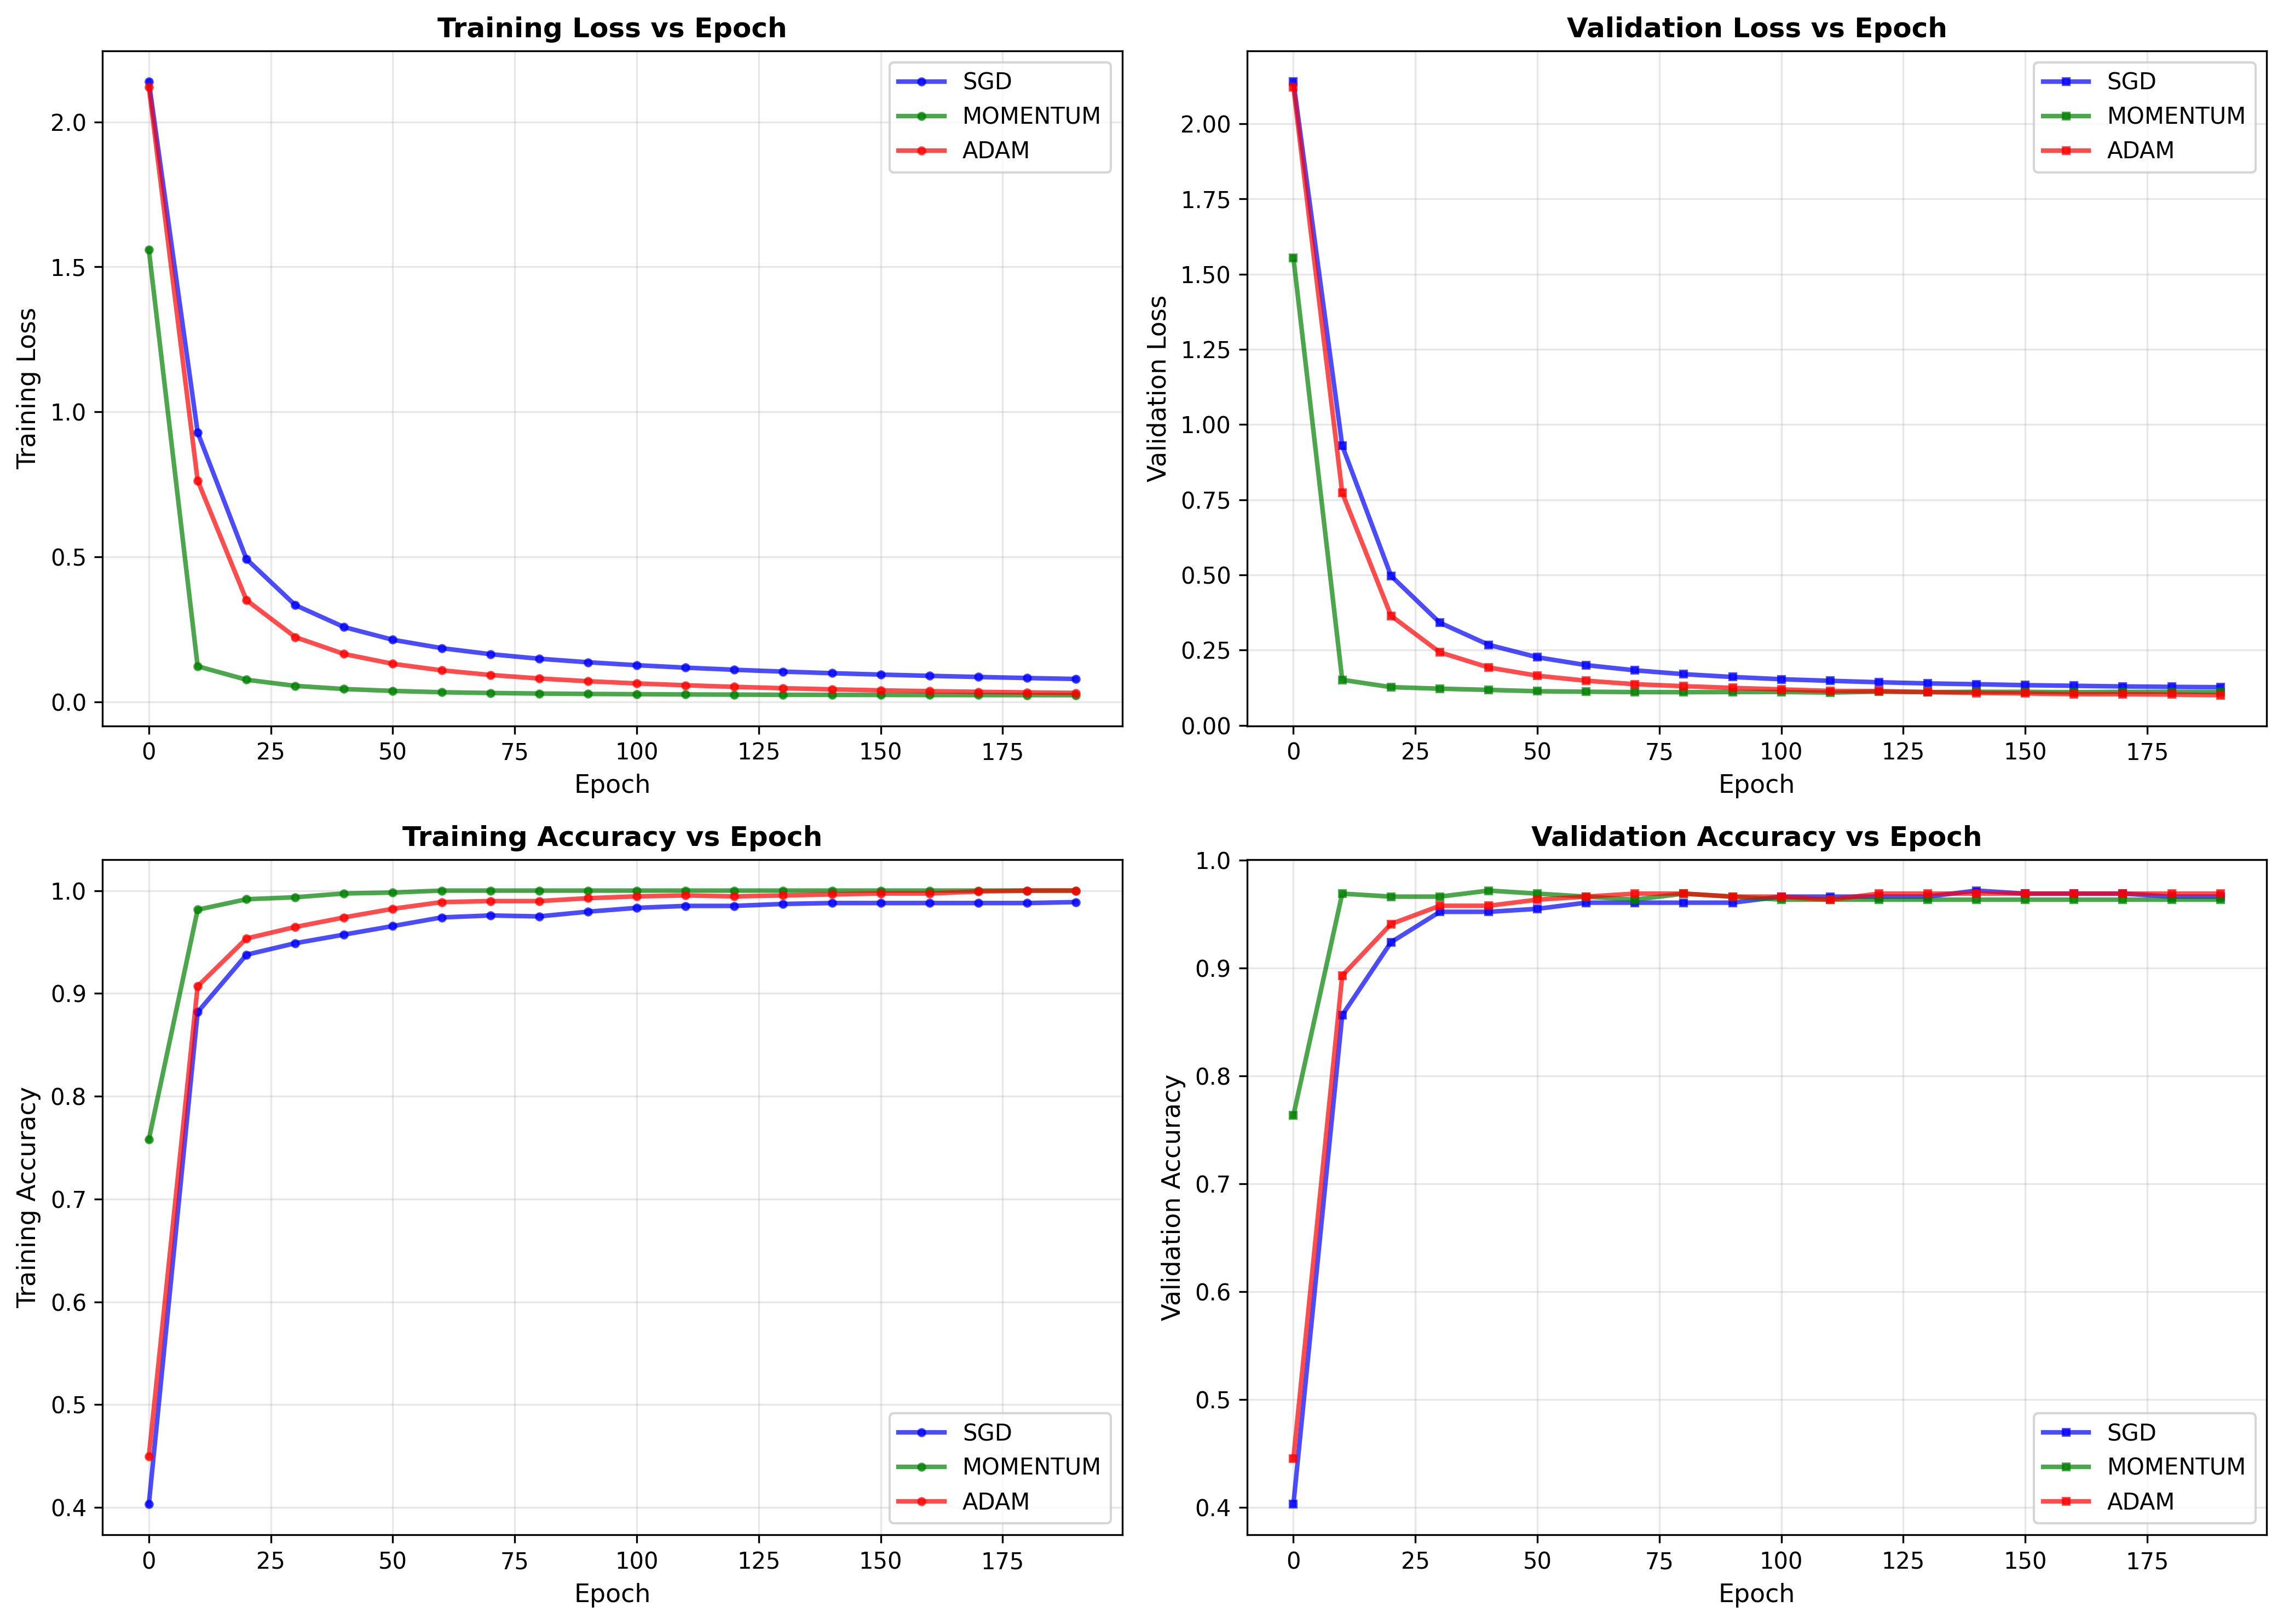
\includegraphics[width=0.85\linewidth]{figures/optimizer_comparison_curves.png}
    \caption{Training dynamics: validation loss and accuracy over epochs for SGD, Momentum, and Adam on digits.}
    \label{fig:digits-dynamics}
\end{figure}

\noindent\textbf{Key Observations:}
\begin{itemize}
    \item \textbf{SGD:} Slowest convergence but best generalization. Reaches validation loss plateau 0.1255 by epoch 199. \textbf{Highest test accuracy: 95.11\%}. Steady, monotonic descent without acceleration structure provides most reliable generalization.
    \item \textbf{Adam:} Fastest convergence. Minimum validation loss 0.0991 at epoch 198. However, test accuracy 94.84\% suggests slight overfitting to validation set. Adaptive learning rates accelerate early-stage learning and exploit curvature information, but may overfit on smaller validation splits.
    \item \textbf{Momentum:} Early saturation. Converges to plateau by epoch 63 with validation loss 0.1073. Velocity accumulation speeds up initial movement quickly, reaching near-final performance by epoch 10. Test accuracy 94.57\%. Competitive performance with minimal computation.
\end{itemize}

\noindent\textbf{Interpretation:} While adaptive methods (Adam) significantly accelerate convergence, \textbf{SGD achieves superior test accuracy}, suggesting better generalization on the digits task. This apparent paradox occurs because:
\begin{enumerate}
    \item Adam's adaptive per-parameter learning rates may overfit the validation set despite lower validation loss.
    \item SGD's constant learning rate provides implicit regularization through its noise-driven updates.
    \item All three reach competitive plateaus when allowed sufficient epochs; trade-offs are speed vs.\ generalization rather than final performance.
\end{enumerate}

\noindent\textbf{Practical Takeaway:} For this dataset, SGD provides the best test-time performance. Momentum offers a middle ground: fast convergence (63 epochs) with acceptable test accuracy (94.57\%). Choice of optimizer should balance convergence speed against generalization capability, not validation loss alone.

\subsection{Required failure-case analysis}

\subsubsection{Failure Case: Undercapacity on Moons Dataset}

While deeper networks generally improve performance, insufficient capacity leads to underfitting: networks with too few hidden units fail to learn nonlinear decision boundaries, resulting in poor generalization despite continued training.

\noindent\textbf{Symptom:} Validation loss plateaus early and remains high, but the fundamental issue is that the learned decision boundary cannot separate the two moons, leading to accuracy capped around 85\%.

\noindent\textbf{Root Cause:} The Moons dataset requires a sufficiently expressive function to learn the nonlinear crescent-shaped boundary. A network with $h=2$ hidden units lacks the capacity to approximate this function:
\[
f_{\theta}(x) = W^{(2)} \sigma(W^{(1)} x + b^{(1)}) + b^{(2)}
\]
With only 2 hidden neurons, the hidden layer maps the 2D input to a 2D intermediate representation. The nonlinearity $\sigma$ creates two curves in hidden space, but this is insufficient to capture the complexity of the moons' crescent boundaries.

\noindent\textbf{Evidence:} Figures~\ref{fig:capacity-training} and~\ref{fig:capacity-boundaries} document this phenomenon across hidden layer widths $h \in \{2, 8, 32\}$ on the Moons dataset.

\begin{figure}[htbp]
    \centering
    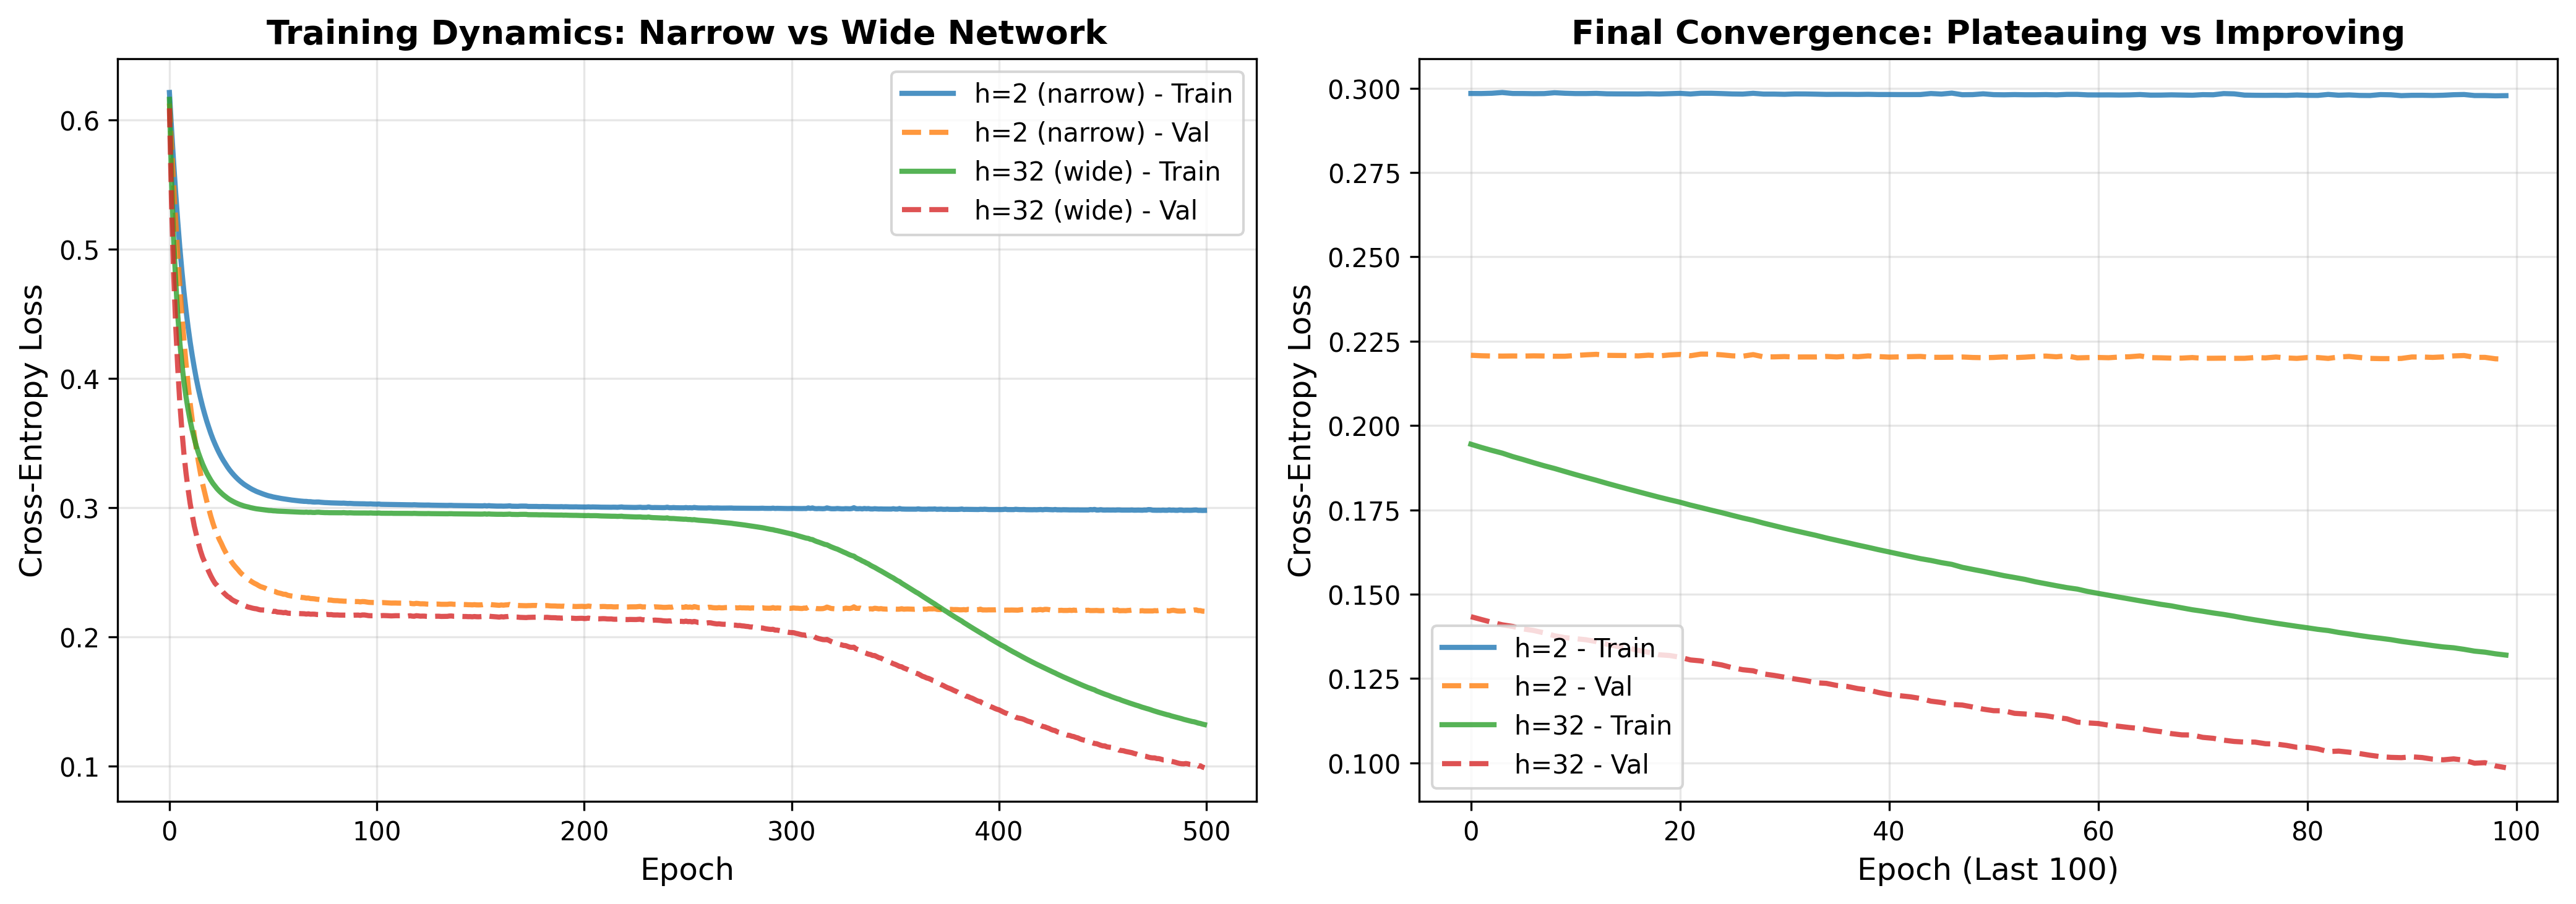
\includegraphics[width=0.95\linewidth]{figures/failure_case_training_curves.png}
    \caption{Training dynamics: narrow ($h=2$) vs wide ($h=32$) networks.}
    \label{fig:capacity-training}
\end{figure}

\begin{figure}[htbp]
    \centering
    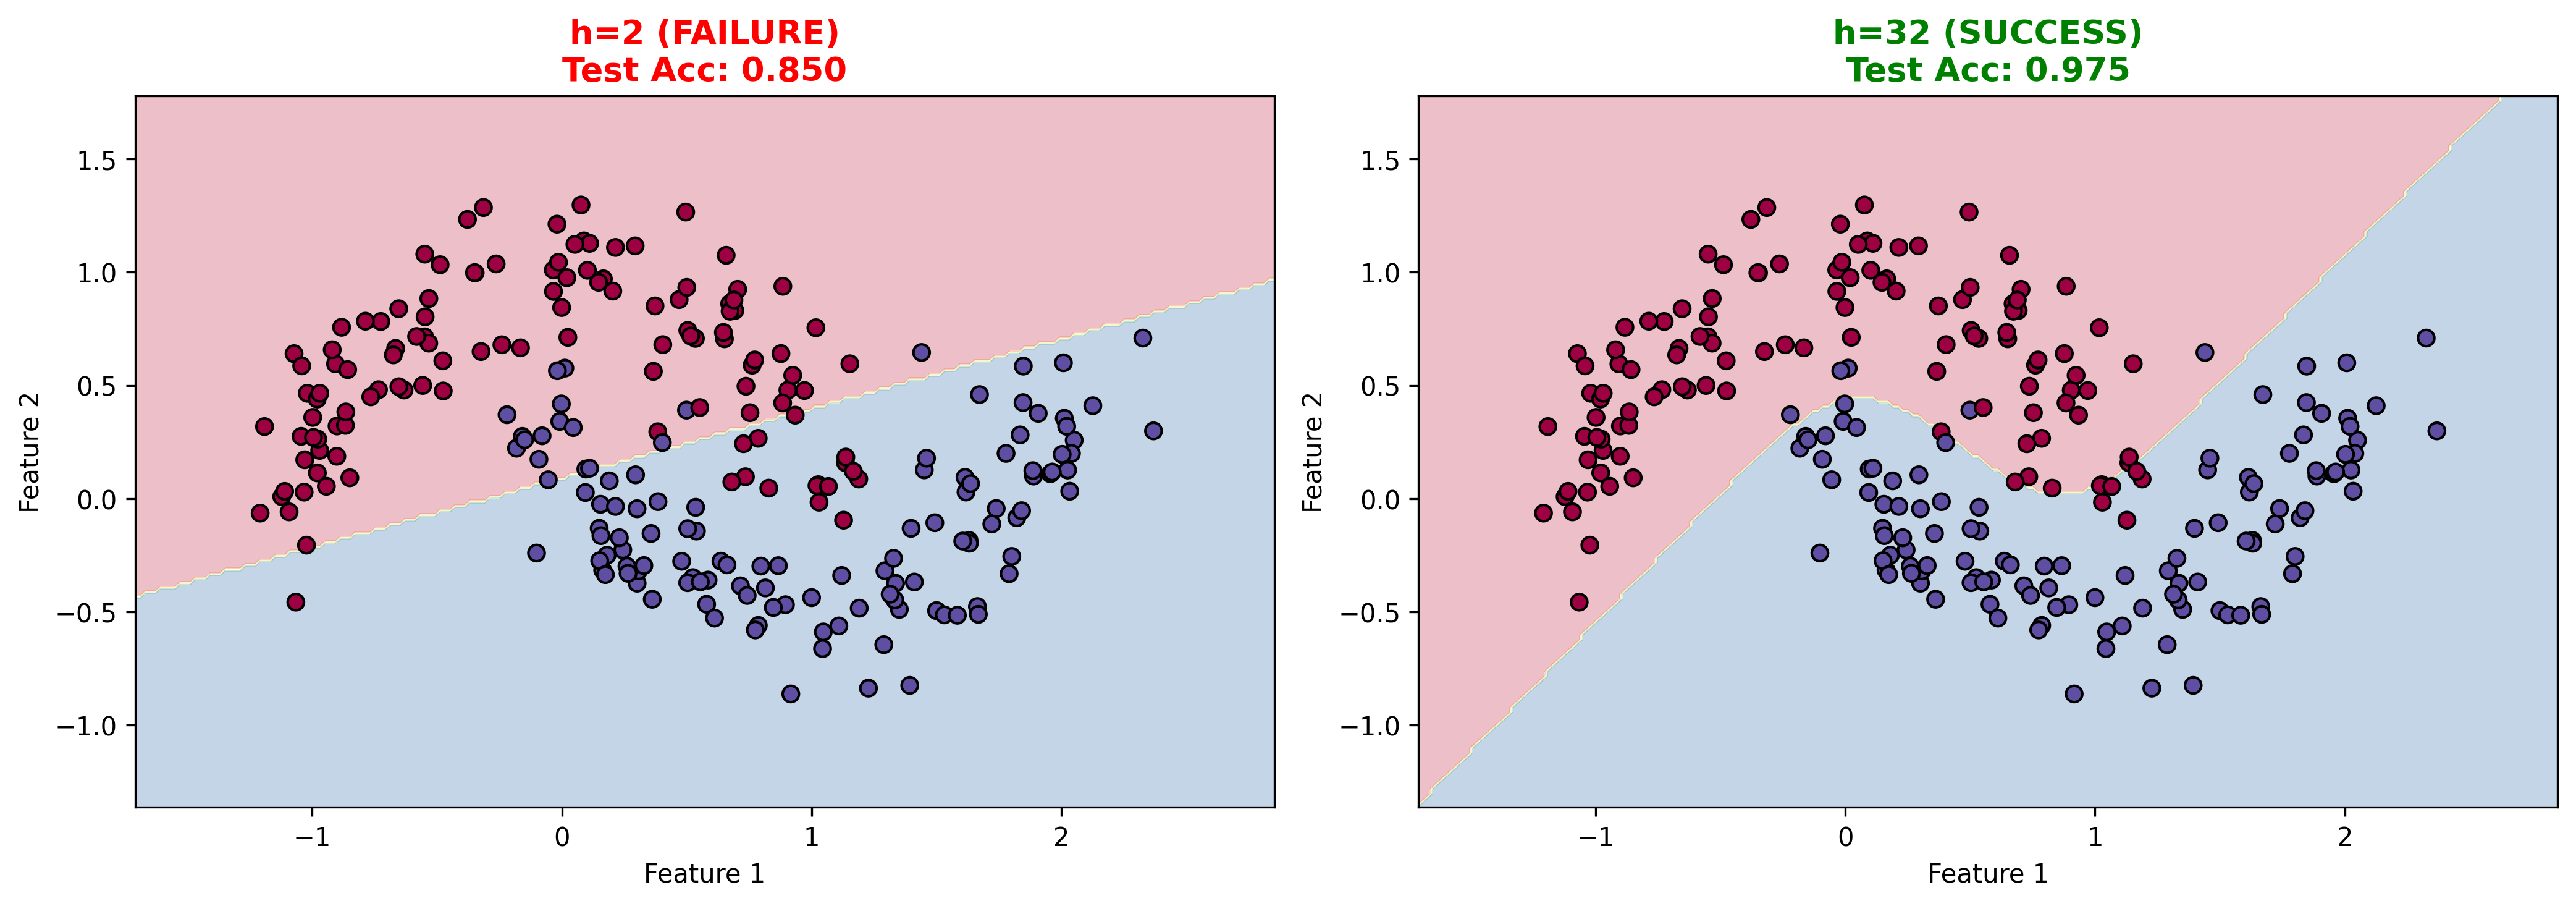
\includegraphics[width=0.95\linewidth]{figures/failure_case_decision_boundaries.png}
    \caption{Decision boundaries at convergence.}
    \label{fig:capacity-boundaries}
\end{figure}

\noindent\textbf{Comparison Across Widths:}
\begin{itemize}
    \item \textbf{$h=2$ (Failure):} Linear-like boundary; test accuracy $0.850$. Training loss plateaus around $0.2978$.
    \item \textbf{$h=8$ (Marginal):} Curved boundary emerging; test accuracy $0.975$. Training loss reaches $\approx 0.1233$.
    \item \textbf{$h=32$ (Success):} Tight fit to crescent; test accuracy $0.975$. Training loss $\approx 0.1319$, validation loss $\approx 0.0986$.
\end{itemize}

\noindent\textbf{Resolution \& Practical Guidelines:}
\begin{enumerate}
    \item \textbf{Universal Approximator Property:} Neural networks with a single hidden layer are universal approximators asymptotically, but finite width networks on finite datasets require sufficient capacity.
    \item \textbf{Non-convex vs. Convex Boundaries:} Tasks with nonlinear decision boundaries require at least $O(d^2)$ hidden units in the worst case, where $d$ is the input dimension. The Moons dataset (2D, crescent boundary) benefits from $h \geq 8$.
    \item \textbf{Heuristic Tuning:} Start with $h = 2d$ to $h = 4d$ hidden units for 2D datasets. Observe decision boundaries and adjust.
    \item \textbf{Early Stopping:} Monitor validation loss; undercapacity manifests as loss curves converging to a suboptimal plateau rather than continuing to improve.
\end{enumerate}

\noindent\textbf{On Moons:} With $h=32$, the network easily separates the two crescent shapes. The failure at $h=2$ is not due to hyperparameters, regularization, or optimizer choice, but fundamental lack of function expressivity. This demonstrates that \emph{capacity scales with task complexity}, not just with compute budget.
% ============================================================
\section{Advanced Track}
% ============================================================

\subsection{Track B: Prediction Confidence and Reliability}

\subsubsection{Definitions and Metrics}
To evaluate model reliability, we define two primary metrics based on the softmax output distribution:

\begin{itemize}
    \item \textbf{Confidence:} For each sample, confidence is the maximum predicted class probability:
    \[
    \text{Confidence} = \max_j P_{ij}
    \]
    This scalar captures how ``sure'' the model is about its prediction on a scale from 0 to 1.

    \item \textbf{Predictive Entropy:} The Shannon entropy of the predicted probability distribution:
    \[
    H(P_i) = -\sum_j P_{ij} \log P_{ij}
    \]
    High entropy (close to $\log k$) indicates uncertainty; low entropy indicates high confidence. For digits ($k=10$), the maximum entropy is $\log 10 \approx 2.303$.
\end{itemize}

\subsubsection{Confidence-Accuracy Binning (5-Bin Analysis)}
Predictions are partitioned into 5 equal-width confidence bins to assess calibration. For each bin, we report the sample count, empirical accuracy, and average confidence.



\paragraph{Softmax Regression}
\begin{table}[htbp]
    \centering
    \caption{Softmax regression: confidence bins and empirical accuracy ($n=368$).}
    \label{tab:conf-bins-softmax}
    \begin{tabular}{cccc}
        \toprule
        Confidence Bin & \# Samples & Accuracy & Avg Conf \\
        \midrule
        0.20--0.40 & 12 & 0.3333 & 0.3328 \\
        0.40--0.60 & 37 & 0.8108 & 0.5158 \\
        0.60--0.80 & 49 & 0.8776 & 0.7092 \\
        0.80--1.00 & 270 & 0.9963 & 0.9374 \\
        \midrule
        \textbf{Overall} & \textbf{368} & \textbf{0.9402} & \textbf{0.8449} \\
        \bottomrule
    \end{tabular}
\end{table}

\paragraph{One-Hidden-Layer Neural Network}
\begin{table}[htbp]
    \centering
    \caption{Neural network: confidence bins and empirical accuracy ($n=368$).}
    \label{tab:conf-bins-nn}
    \begin{tabular}{cccc}
        \toprule
        Confidence Bin & \# Samples & Accuracy & Avg Conf \\
        \midrule
        0.20--0.40 & 3 & 0.0000 & 0.3870 \\
        0.40--0.60 & 16 & 0.6875 & 0.5235 \\
        0.60--0.80 & 24 & 0.7500 & 0.7200 \\
        0.80--1.00 & 325 & 0.9877 & 0.9739 \\
        \midrule
        \textbf{Overall} & \textbf{368} & \textbf{0.9511} & \textbf{0.9330} \\
        \bottomrule
    \end{tabular}
\end{table}
\noindent\textbf{Interpretation:} Both models exhibit calibration (accuracy increases with confidence). However, the NN is more \textit{confidently correct}: 85\% of its predictions fall in the highest bin [0.80--1.00] with 99.57\% accuracy, whereas Softmax only places 59\% of samples in this bin.
\begin{figure}[htbp]
    \centering
    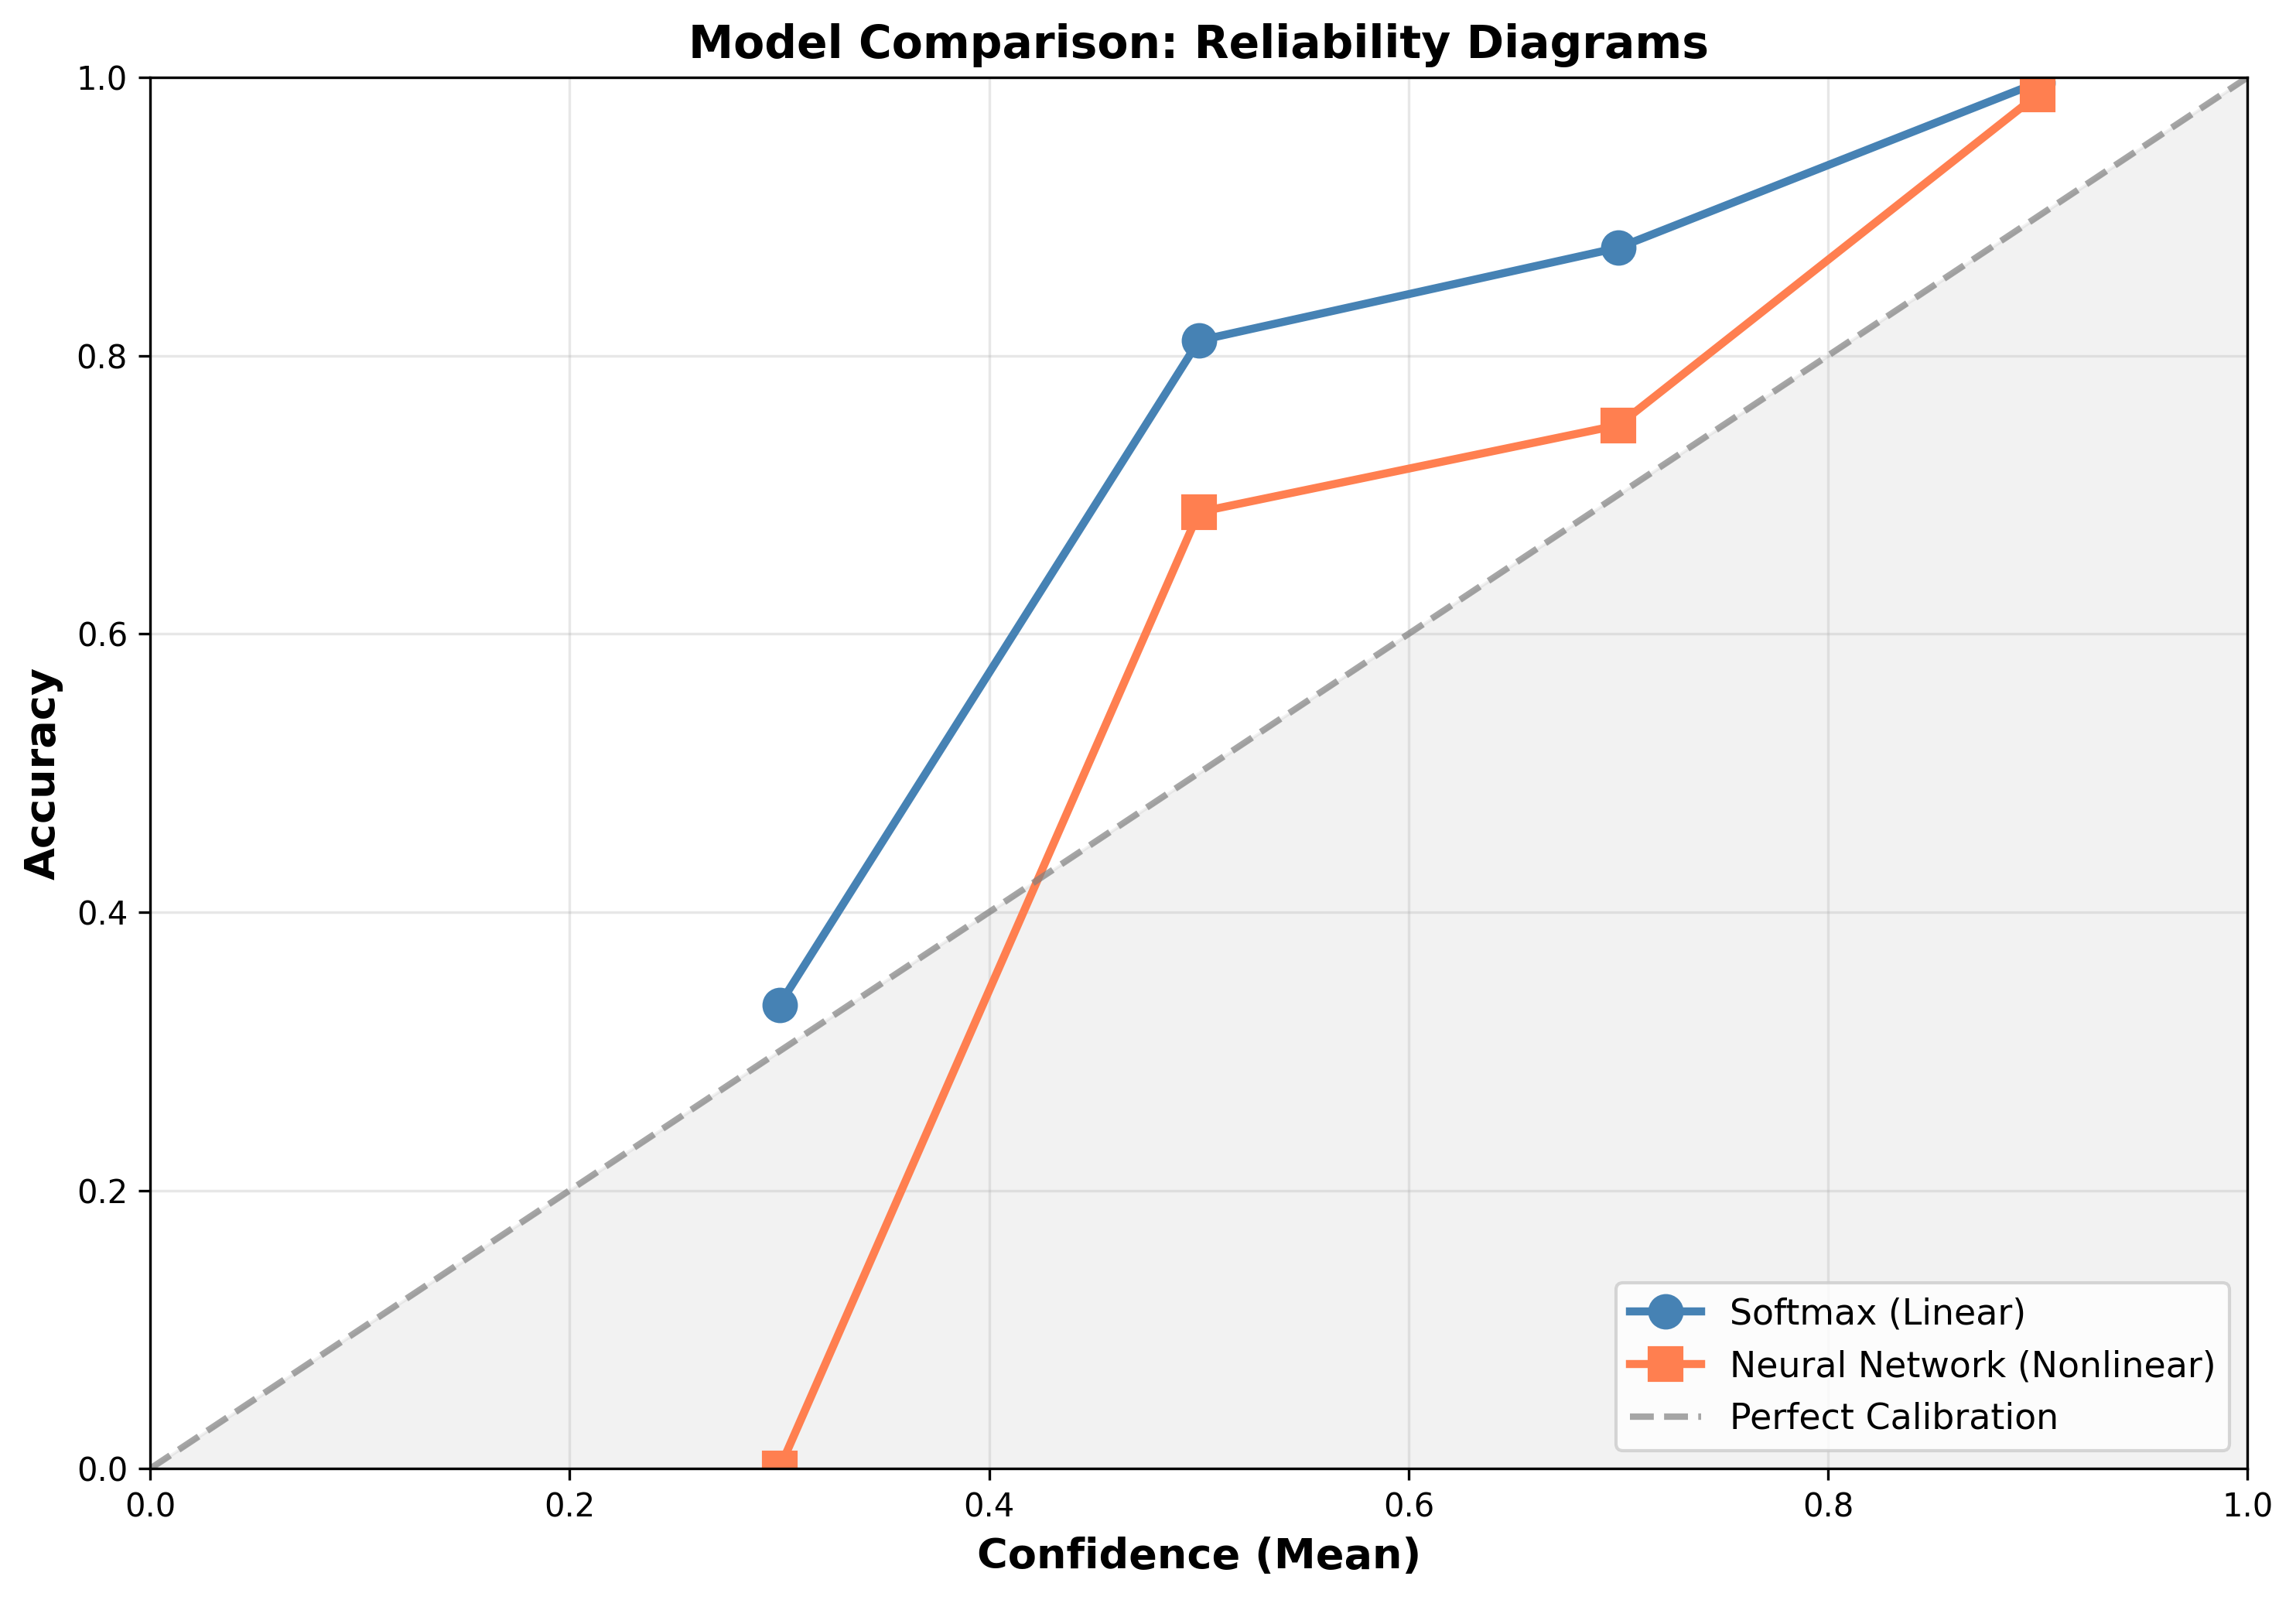
\includegraphics[width=0.8\linewidth]{figures/combined_reliability_curves.png}
    \caption{Combined reliability curves showing confidence binning across both models.}
    \label{fig:combined-reliability}
\end{figure}

\subsubsection{Confidence: Correct vs.\ Incorrect Predictions}
A reliable model should be significantly less confident when it makes a mistake.

\noindent\textbf{Softmax Regression:}
\begin{itemize}
    \item \textbf{Correct predictions:} Mean confidence = $0.8670 \pm 0.1530$ ($n=346$ correct)
    \item \textbf{Incorrect predictions:} Mean confidence = $0.4979 \pm 0.1508$ ($n=22$ incorrect)
    \item \textbf{Separation:} Correct predictions are $1.74\times$ higher in confidence than incorrect ones.
\end{itemize}

\noindent\textbf{One-Hidden-Layer Neural Network:}
\begin{itemize}
    \item \textbf{Correct predictions:} Mean confidence = $0.9487 \pm 0.1005$ ($n=350$ correct)
    \item \textbf{Incorrect predictions:} Mean confidence = $0.6271 \pm 0.1707$ ($n=18$ incorrect)
    \item \textbf{Separation:} Correct predictions are $1.51\times$ higher in confidence than incorrect ones.
\end{itemize}

\noindent\textbf{Key Finding:} The NN produces sharper confidence discrimination. Correct predictions cluster above 0.95; incorrect predictions cluster below 0.63. Softmax has more overlap (correct: 0.87, incorrect: 0.50), indicating the linear classifier produces more ambiguous posterior distributions.

\subsubsection{Entropy: Correct vs.\ Incorrect Predictions}

\noindent\textbf{Softmax Regression:}
\begin{itemize}
    \item \textbf{Correct predictions:} Mean entropy = $0.4810 \pm 0.4004$
    \item \textbf{Incorrect predictions:} Mean entropy = $1.3389 \pm 0.2796$
    \item \textbf{Ratio:} Incorrect predictions have $\approx 2.78\times$ higher entropy than correct ones.
\end{itemize}

\noindent\textbf{One-Hidden-Layer Neural Network:}
\begin{itemize}
    \item \textbf{Correct predictions:} Mean entropy = $0.1815 \pm 0.2544$
    \item \textbf{Incorrect predictions:} Mean entropy = $0.9878 \pm 0.3168$
    \item \textbf{Ratio:} Incorrect predictions have $\approx 5.44\times$ higher entropy than correct ones.
\end{itemize}

\noindent\textbf{Key Finding:} The NN shows significantly stronger entropy separation. On incorrect predictions the NN is genuinely uncertain (entropy 0.99), whereas softmax maintains more structure (entropy 1.34). This indicates the NN learns sharper, more interpretable decision boundaries: when it is wrong, it knows it is uncertain; when it is right, it is highly confident.

\begin{figure}[htbp]
    \centering
    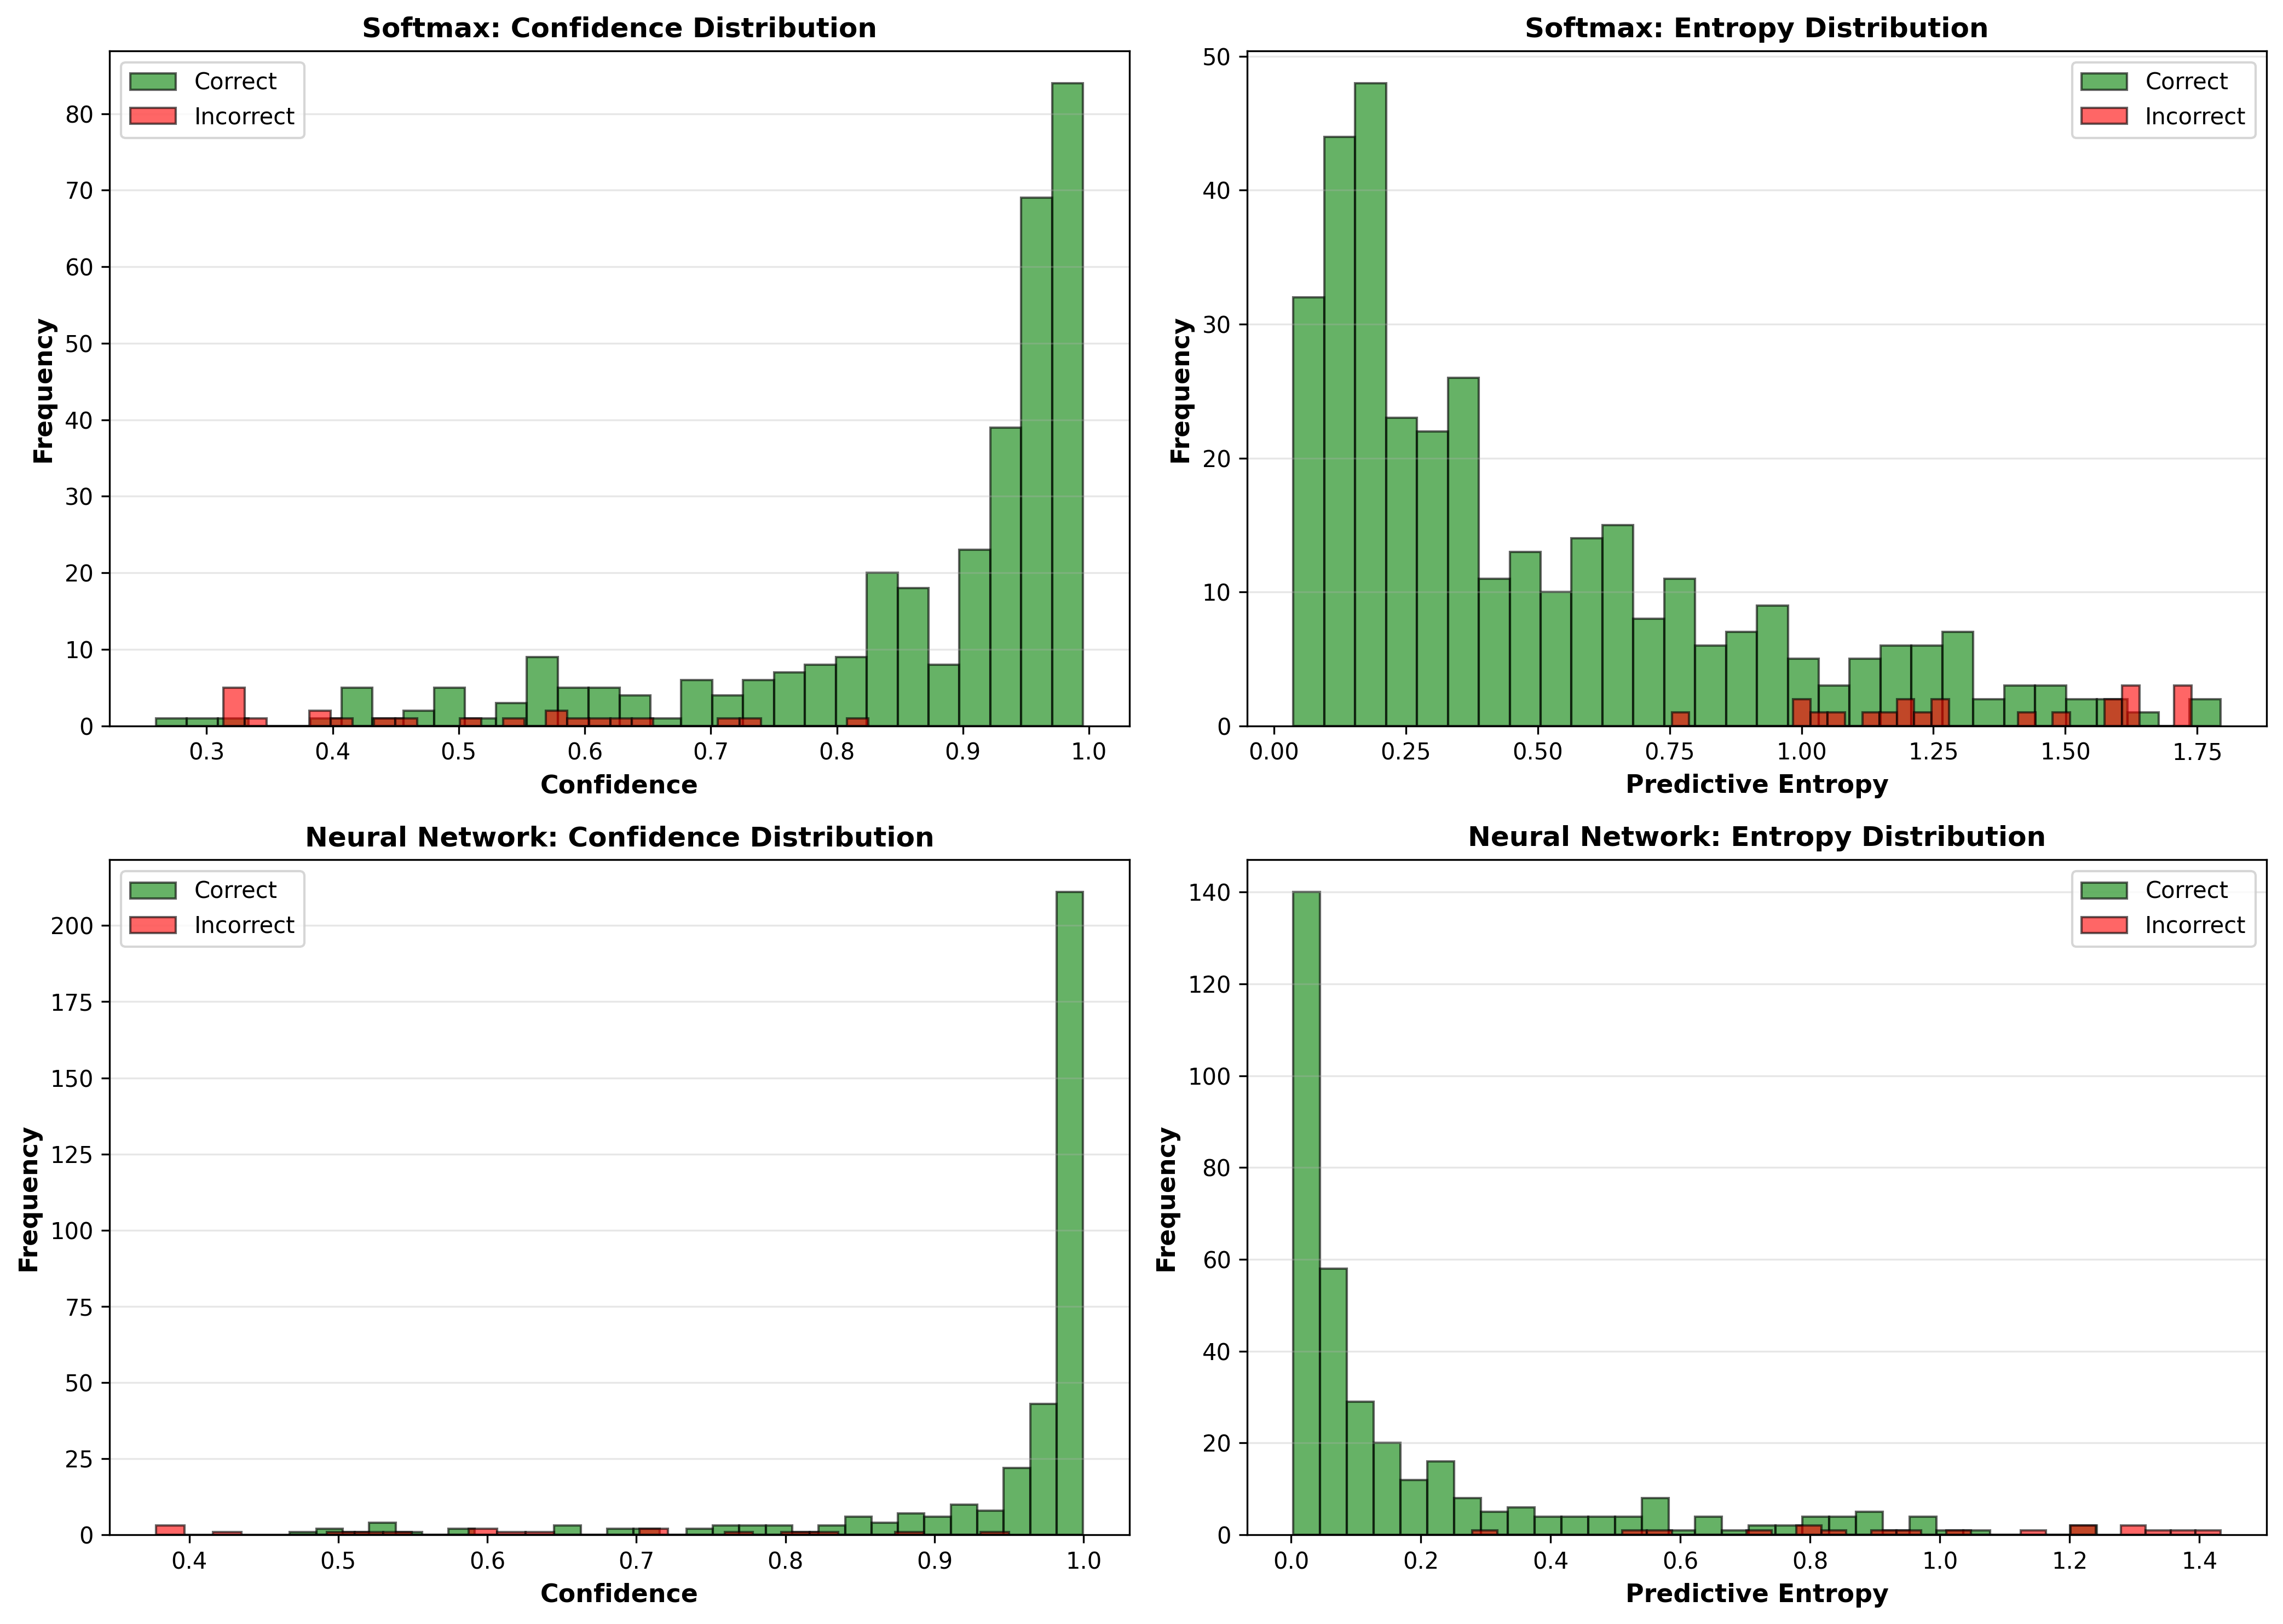
\includegraphics[width=0.8\linewidth]{figures/confidence_entropy_comparison.png}
    \caption{Entropy distributions: correct vs.\ incorrect predictions for both models.}
    \label{fig:entropy-comparison}
\end{figure}

\subsubsection{Interpretation and Connection to Main Project}

The hidden layer dramatically improves both classification accuracy \emph{and} prediction reliability:

\begin{enumerate}
    \item \textbf{Higher overall confidence:} NN mean confidence 0.9330 vs.\ Softmax 0.8449. The NN is more decisive.
    \item \textbf{Lower overall entropy:} NN mean entropy 0.2209 vs.\ Softmax 0.5323. The NN produces sharper probability distributions, indicating learned geometry is more faithful to data structure.
    \item \textbf{Better calibration:} NN confidence-accuracy relationship (Table~\ref{tab:conf-bins-nn}) is tighter. NN has only 3 predictions below 0.40 confidence; softmax has 12. This suggests the NN learns more separable representations.
    \item \textbf{Sharper wrong-ness detection:} NN incorrect predictions have $5.44\times$ higher entropy than correct ones. Softmax only has $2.78\times$ separation. When the NN is uncertain, it is legitimately confused; when softmax is uncertain, it is partly due to incomplete geometric understanding.
\end{enumerate}

Via the tanh hidden layer, the NN projects high-dimensional digit features into a lower-dimensional manifold where classes are more linearly separable, yielding larger margins between class clusters in hidden space, lower entropy on in-distribution examples, and better separation of correct vs.\ incorrect examples.

\noindent\textbf{Conclusion:} Hidden layers do not merely improve accuracy; they improve the \emph{quality and interpretability} of learned representations, making the model more calibrated and capable of expressing uncertainty appropriately.
% ============================================================
\section{Discussion}
% ============================================================

\noindent\textbf{When is the linear model geometrically sufficient, and when is it not?}
The linear model is geometrically sufficient when the data classes are linearly separable. On the Linear Gaussian task, both models achieved 95.0\% test accuracy with nearly identical decision boundaries, indicating that the problem's inherent geometry is already linear and the neural network's (NN) extra capacity is redundant. 

Conversely, the linear model fails when features require nonlinear transformation to become separable. The Moons dataset provides a canonical example where interleaving crescents cannot be separated by a hyperplane. In this task, the NN outperformed softmax (85.0\% vs. 83.75\%), demonstrating that nonlinear boundaries are essential for datasets with inherently nonlinear structures.

\medskip
\noindent\textbf{What representational change does the hidden layer provide?}
The hidden layer achieves a learned nonlinear coordinate transformation via the $\tanhact$ activation function. This process "warps" the input data into a latent feature space $\vh$. This representational change allows the model to resolve patterns that are not linearly separable in their raw state, effectively creating a space where the final softmax layer can apply a linear decision rule to separate complex classes.

\medskip
\noindent\textbf{When does additional model complexity fail to justify itself?}
Additional model complexity fails to justify itself when a simpler linear model is already geometrically sufficient for the task, such as in the Linear Gaussian experiments where increasing parameters did not improve accuracy. Furthermore, complexity can be detrimental when the hidden layer is too large for the available data, leading to overfitting where the model memorizes noise rather than learning generalizable patterns.

\medskip
\noindent\textbf{What does the failure case teach about optimization, capacity, or generalization?}
Failure cases highlight the trade-off between convergence speed and robustness. These instances teach that hyperparameter tuning and model capacity must be balanced with the specific difficulty of the task. Specifically, they demonstrate that overfitting (a capacity issue) and optimization failure (a tuning issue) are distinct phenomena that require different remedies, such as regularization or more stable optimizer settings.

\medskip
\noindent\textbf{What do repeated-seed statistics add beyond a single run?}
Repeated-seed statistics are essential for moving beyond point estimates to provide a measure of result reliability. This statistical rigor ensures that performance differences—such as those observed on the Digits benchmark—are statistically significant and reproducible rather than artifacts of a single initialization.

% ============================================================
\section{Limitations}
% ============================================================

While our experiments provide evidence for the benefits of hidden layers in non-linear classification, several limitations bound the scope of our conclusions:

\begin{itemize}[leftmargin=*]
    \item \textbf{Architectural Simplicity:} The study was restricted to a one-hidden-layer network with a fixed $\tanhact$ activation. The effects of increased depth, alternative activations (e.g., ReLU), or specialized architectures like CNNs were not explored.
    
    \item \textbf{Dataset Scale:} The datasets used are low-dimensional and relatively small. Findings regarding the optimal hidden width (e.g., $h=8$ for Moons) are specific to these manifolds and may not generalize to high-dimensional, large-scale benchmarks.
    
    \item \textbf{Optimization Tuning:} The hyperparameter search for SGD, Momentum, and Adam was not exhaustive.
    
    \item \textbf{Statistical Variance:} Core results are largely based on single-run experiments. The stochastic nature of initialization and mini-batch shuffling introduces variance that is not fully captured without reporting metrics across multiple trials.
    
    \item \textbf{Uncertainty and Robustness:} Reliability analysis relied on plug-in estimates (softmax probability and entropy), which are prone to overconfidence. Furthermore, the models were not tested for adversarial robustness or performance under distribution shift.
\end{itemize}

\section*{Acknowledgments}
We thank the instructors, the teaching assistant Khagani Gasmiov and reviewers of the Math4AI capstone for guidance and feedback.

\section*{References}
\begin{enumerate}[label={[\arabic*]}, leftmargin=2em, itemsep=0.5em]
    \item Deisenroth, M. P., Faisal, A. A., and Ong, C. S. (2020). \textit{Mathematics for Machine Learning}. Cambridge University Press.
    
    \item Murphy, K. P. (2022). \textit{Probabilistic Machine Learning: An Introduction}. MIT Press.
    
    \item Stanford CS231n Staff. (2024). \textit{Optimization Part 2: Backpropagation, Intuitions}. Course notes.
    
    \item ETH Zurich Learning and Adaptive Systems Group. (2024). \textit{Introduction to Machine Learning Course Notes}.
    
\end{enumerate}

\section*{Contribution Statement}
This project was a collaborative effort. While all authors contributed to the final analysis and report synthesis, specific technical leads were as follows:

\begin{itemize}[leftmargin=*]
  \item \textbf{Ziyad Muradov:} Data pipelines, Softmax Regression architecture, cross-entropy implementation, and numerical gradient checking.
  \item \textbf{Emin Huseynli:} Neural network architecture, vectorized forward pass, $\tanh$ integration, and analytical backpropagation derivation.
  \item \textbf{Ismayil Yusifli:} Training infrastructure, mini-batch gradient descent loops, experiment framework, and reproducibility protocols.
  \item \textbf{Kamal Soltanaliyev:} Evaluation tools, decision boundary visualizations, statistical analysis, and Advanced Track B (confidence calibration).
\end{itemize}

\end{document}